% !TeX spellcheck = en_GB
% ***************************************************** %
\section{Mini-batch gradient descent variants}
% ***************************************************** %

In this section we tackle the algorithmic part, the SGD-type chosen is the Mini-batch Gradient Descent where the mini-batch size $M$ is greater than 1 and much less than the dataset size, i.e. $1<\abs{B_t}=M\ll N$. For simplicity, we will call it SGD anyway.

The basic SGD performs steps of the form
\begin{equation}\label{eq:sgd_step}
w^{k+1}=w^k+\alpha_kd_k,\quad d_k=-\nabla f_{i_k}(w^k)
\end{equation}
where the direction $d_k$ is equal to the \emph{anti-gradient} evaluated on the considered sample (a random mini-batch extracted from the dataset), knowing that $\numberset{E}\bigl[\nabla f_{i_k}(w^k)\bigr]=\nabla\func(w)$, $d_k$ is a \emph{descent direction}. Also due to the global convergence, the algorithm can start from an arbitrary $w^0\in\R^{(p+1)}$.

Using this step-size form, without a line search method for choosing the optimal step-size $\alpha_k$, the objective function value doesn't decrease necessarily at each step, thus making the method \emph{non-monotonous}.

In order to use the SGD algorithm, it is necessary to make further assumptions on the objective function and the gradients (how far the gradient samples are from the \emph{true gradients})
\begin{itemize}
\item the function $f$ in problem~\eqref{eq:opt-prob} has a \emph{finite-sum structure}, that is the common machine learning setting;
\item being a loss function plus a quadratic regularization term, $f$ is bounded below by some value $f^\ast$, we can also take a look at figure~\ref{subfig:log-loss};
\item for some constant $G>0$ the magnitude of all gradients samples are bounded $\forall w\in\R^{(p+1)}$ by $\norma{\nabla f_i(w)}\leq G$;
\item other than twice continuously differentiable, we assume that $f$ has Lipschitz-continuous gradients with constant $L>0$, one can also say that $f$ is $L\text{-smooth}$.
\end{itemize}

Regarding the implementation of the algorithm, it is essential to define a stopping criterion. The first choice is always
\begin{equation}\label{eq:stopping1}
\norma{\nabla\func(w^k)}\leq\epsilon,\quad\epsilon>0
\end{equation}
unless there is a small tolerance $\epsilon$, the algorithm reaches a stationary point.

Other than this, we can add conditions of premature termination like
\begin{itemize}
\item exceeding a threshold for the epochs number $k^\ast$ or function and gradient evaluations;
\item internal failures when computing $w^{k+1}$, for example during the line search.
\end{itemize}


\subsubsection*{Mini-batch gradient}

Now we spend a few words about the computation of the mini-batch gradient evaluated on a point using the pseudo-code notation. Given a mini-batch $B_t$ at iteration $t$ with indices $i_t$ and the previous weights $y_t$, we want to compute
\begin{equation*}
%\begin{split}
%\nabla f_{i_t}(y_t) &= \frac{1}{M}\sum_{j\in B_t}\nabla f_j(y_t)\\
% &= \frac{1}{M}\sum_{j\in B_t}\bigl(x^{(j)}r_j+\lambda y\bigr) \\
% &= \frac{1}{M}\biggl(\sum_{j\in B_t}x^{(j)}r_j+M\lambda y\biggr) \\
% &= \frac{1}{M}\bigl(\underbrace{Xr}_{i_t\in B_t}+\lambda' y\bigr)
%\end{split}
\begin{split}
\nabla f_{i_t}(y_t) &= \frac{1}{M}\sum_{j\in B_t}\nabla f_j(y_t)=\frac{1}{M}\sum_{j\in B_t}\bigl(x^{(j)}r_j+\lambda y\bigr)= \frac{1}{M}\biggl(\sum_{j\in B_t}x^{(j)}r_j+M\lambda y\biggr) \\
 &= \frac{1}{M}\bigl(\underbrace{Xr}_{i_t\in B_t}+\lambda' y\bigr)
\end{split}
\end{equation*}
so we use the same expression as the full gradient except that the dataset matrix contains just the mini-batch samples (and so the $r$ vector), and the regularization coefficient is redefined as $\lambda'=M\lambda$ where $M$ is the size of the considered mini-batch.

% ---------------------------------------------------- %
\subsection{Stochastic gradient descent}
% ---------------------------------------------------- %

The SGD-type variants differs by the selection of the step-size. Particularly the basic version has two possible choices
\begin{itemize}
\item \emph{constant step-size} $\alpha_k=\alpha$;
\item \emph{decreasing step-size} $\alpha_k=\frac{\alpha_0}{k+1}$.
\end{itemize}
the second choice has such form in order to ensure the convergence of the algorithm; this two version are shown in algorithm~\vref{code:SGD-fix-decr}. The iteration~\eqref{eq:sgd_step} sees the index $k$ changed to $t$, the former is the index of the \emph{epochs} while the latter is the index of the mini-batches.

% ---------------------------------------------------- %
\subsubsection{Stochastic line search}
% ---------------------------------------------------- %

Now we move on to the approach by \texttt{bib1}. Other than $\mathcal{L}_0=\set{w\in\R^{(p+1)}\mid\func(w)\leq\func(w^0)}$ being a \emph{compact set}, since the function is coercive (see\dots), the proposed algorithm needs one more assumption, that is, the model is able to \emph{interpolate} the data, this property requires that the gradient w.r.t. each samples converges to zero at the optimal solution
\[
\text{if}\,\,\,w^\ast\mid\nabla\func(w^\ast)=0\Rightarrow\nabla f_i(w^\ast)=0\,\,\,\forall i=1,\dots,N
\]

The proposed approach applies the Armijo line search to the SGD algorithm, specializing the condition of sufficient reduction in the context of finite-sum problems. Referring to the notation in~\eqref{eq:sgd_step}, the \emph{Armijo condition} has the following form
\[
\func(w^{k+1})\leq\func(w^k)+\gamma\alpha_k\nabla\func(w^k)^Td_k\Rightarrow
f_{i_k}(w^{k+1})\leq f_{i_k}(w^k)+\gamma\alpha_k\nabla f_{i_k}(w^k)^Td_k
\]
so, when it comes to SGD we obtain
\begin{equation}\label{eq:armijo-sls}
f_{i_k}\bigl(w^k-\alpha_k\nabla f_{i_k}(w^k)\bigr)\leq f_{i_k}(w^k)-\gamma\alpha_k\nabla\norma{f_{i_k}(w^k)}^2
\end{equation}
as already said, $d_k$ is a \emph{descent direction}. The constant $\gamma$ is an hyper-parameter set to $1/2$ for convergence properties in the strongly-convex case.

As the standard Armijo method, the proposed line search uses a \emph{backtracking} technique that iteratively decreases the initial step-size $\alpha_0$ by a constant factor $\delta$ usually set to $1/2$ until the condition is satisfied.

The authors also gave heuristics in order to avoid unnecessary function evaluations by \emph{restarting} at each iteration the step-size, see algorithm~\vref{code:reset-step}.\footnote{\emph{Iterations} is defined as the total number of mini-batches extracted from the dataset, while one \emph{epoch} is when the entire dataset is passed forward.}

The SGD with Stochastic Line Search is shown in algorithm~\vref{code:SGD-Armijo}.

% ---------------------------------------------------- %
\subsection{Adding momentum term}
% ---------------------------------------------------- %

The iteration performed is still $w^{k+1}=w^k+\alpha_kd_k$ what differs from the basic versions is the direction
\[
d_k=-\bigl((1-\beta)\nabla f_{i_k}(w^k+\beta d_{k-1})\bigr)
\]
in a finite-sum problem the momentum term must be selected from a specific range $\beta\in(0,1)$, the algorithm is called SGDM, the resulting iteration
\begin{equation}\label{eq:sgdm-step}
w^{k+1}=w^k-\alpha_k\bigl((1-\beta)\nabla f_{i_k}(w^k+\beta d_{k-1})\bigr)
\end{equation}
which is applied in algorithm~\vref{code:SGDM}.

As the paper \texttt{bib2} says, when using the momentum term together with a line search, $\beta$ complicates the selection of a suitable step-size; using the algorithm~\ref{code:SGD-Armijo}, the approach is not robust to the choice of the momentum term.

Like the stochastic line search approach in section ..., the Armijo condition added to the SGDM algorithm has the form
\begin{equation}\label{eq:armijo-sgdm}
f_{i_k}(w^k+\alpha_kd_k)\leq f_{i_k}(w^k)-\gamma\alpha_k\nabla f_{i_k}(w^k)^T\bigl((1-\beta)\nabla f_{i_k}(w^k+\beta d_{k-1})\bigr)
\end{equation}
placing $d_{i_k}=-\nabla f_{i_k}(w^k)$ we obtain the equation~\eqref{eq:armijo-sls}.

The problem is that $\nabla f_{i_k}(w^k)^Td_{i_k}<0$ isn't always guaranteed, i.e. the direction is not descent, therefore the line search doesn't converge. There are thus two situations that can be resolved as follows
\begin{center}
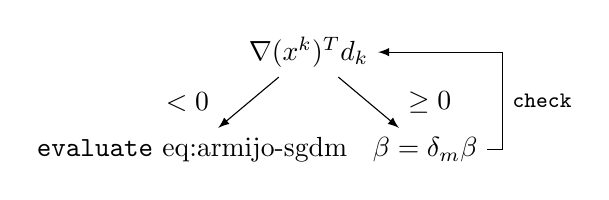
\begin{tikzpicture}
\node (A) at (0,0) {$\nabla\func(x^k)^Td_k$};
\node (B) at (-140:5.5em) {\texttt{evaluate}~\eqref{eq:armijo-sgdm}};
\node (C) at (-40:5.5em) {$\beta=\delta_m\beta$};
\draw[-latex] (A) -- node[left=2.5ex] {$<0$} (B);
\draw[-latex] (A) -- node[right=2.5ex] {$\geq0$} (C);
%\draw[-latex, bend right=55] (C.east) to (A.east);
\draw[-latex] (C.east) -- ++(0.2,0) -- node[right, font=\footnotesize] {\texttt{check}} ++(0,{5.5em*sin(40)}) -- (A.east);
\end{tikzpicture}
\end{center}
in algorithmic terms, while the direction is not descent, damp the momentum term by a factor $\delta_m$ usually set to $1/2$. Using this procedure, a descent direction $d_{i_k}$ is guaranteed, and is called \emph{momentum correction}, see algorithm~\vref{code:MSL-SGDM-C}.

This procedure can be expensive, so the paper suggests another approach called \emph{momentum restart}, when descent direction condition for $d_k$ isn't satisfied, the procedure sets $d_{k-1}=d_0=0$, see algorithm~\vref{code:MSL-SGDM-R}.
